\chapter{Opis projektnog zadatka}
		
		
Cilj ovog projekta je razvoj programske podrške za stvaranje interaktivne web aplikacije „GlobeRunner“  koja omogućuje igračima međusobnu borbu kartama koje su sakupili na različitim stvarnim lokacijama svijeta. Moguće lokacije koje igrači mogu posjetiti su gradovi, naselja, vrhovi planina, umjetničke instalacije, izvori vode, planinarski domovi i sl.
Svaki se neregistrirani korisnik za pristup aplikaciji može prijaviti u već postojeći račun pri čemu je potrebno upisati korisničko ime i lozinku ili stvoriti novi račun. Za stvaranje novog računa potrebni su sljedeći podaci:
		\begin{packed_item}
			\item {Korisničko ime}
			\item {Fotografija}
			\item {E - mail adresa}
			\item {Lozinka}
		\end{packed_item}
		
Pri registraciji korisnik može odabrati jednu od uloga: igrač ili kartograf. Naknadno se može dodijeliti uloga administratora. Registracija nije prihvatljiva ako je zadano korisničko ime ili e – mail adresa već postojećeg računa ili nepostojeća e – mail adresa. Nakon popunjavanja podataka za registraciju korisniku se na e – mail šalje link kojim potvrđuje svoj račun. Ako se korisnik odluči za ulogu kartografa dodatno je potrebna potvrda administratora te dodatni podaci za primanje naknade:
		\begin{packed_item}
			\item {IBAN računa za uplatu}
			\item {Fotografija osobne iskaznice}
		\end{packed_item}
	

Administrator će odbiti registraciju kartografa ako je predan nepostojeći IBAN ili je utvrdio neispravnost podataka.\\

\textit {\underbar{Karta (Lokacija)}} je glavni element igre kojom se igrači međusobno bore. Svaka karta ima naziv, opis, fotografiju i jačinu. Što je lokacija šira i lakše dostupna, to je karta slabija (npr. gradovi su slabiji od muzeja u tim gradovima). Karta nakon svake upotrebe slabi do nule nakon čega više nije upotrebljiva. Cilj ovoga je potaknuti igrače da putuju svijetom i skupljaju što više karata.\\
 
\textit {\underbar{Igrač}} je svaki korisnik koji aktivno skuplja karte i sudjeluje u borbama. Za ispravno i uspješno korištenje aplikacije mora imati uključen GPS.
Za vrijeme igre igraču su vidljivi svi aktivni igrači unutar 50 km s kojima može ući u borbu. Omogućeno mu je pregledavanje profila igrača što uključuje sakupljene karte, poredak u odnosu na ostale igrače te statistiku temeljenu na zadnjih 10 borbi.
Također može pregledati globalnu statistiku svih odigranih borbi, globalnu statistiku svih lokacija te poredak ostalih igrača. Igrač može sakupljati nove karte tako što posjeti određenu lokaciju, također ako je dovoljno iskusan i visoko na poretku može prijaviti novu lokaciju u blizini dodavajući sve potrebne podatke lokacije. Prije ulaska u borbu s drugim igračem, igrač može birati skup karata s kojim će se boriti.\\

\textit {\underbar{Borba}} se odvija tako što 2 igrača naizmjenice vuku po jednu kartu iz svog skupa. Karta s većom jačinom pobjeđuje te igrač čija je karta pobijedila dobiva bod. Nakon što su sve karte iskorištene igrač s više bodova pobjeđuje borbu.\\

\textit {\underbar {Kartograf}} održava i uređuje bazu sustava u koju zapisuje nove prijavljene lokacije.
Kartograf mora osigurati ispravnost zahtjeva za prijavu novih lokacija koje su igrači podnijeli. Može pristupiti popisu svih trenutno aktivnih zahtjeva. Lokacije za koje su podneseni zahtjevi vidljivi su mu na karti a on ih može prihvatiti, urediti, odbiti ili označiti da je potrebna potvrda s terena. Ako označi da je potrebna potvrda s terena može dodatno odlučiti da će ih on sam potvrditi i odlazi na lokaciju najkraćim putem.\\

\textit {\underbar {Administrator}} je korisnik s najviše ovlasti u igri koji ima pristup gotovo svim dijelovima sustava. Sadrži sve mogućnosti koje posjeduju igrači te kartografi, a uz to dodatno mora potvrditi svaku novu registraciju kartografa, može vidjeti i uređivati popis svih korisnika te njihovih osobnih podataka, privremeno isključiti igrača iz igre te može uređivati i postojeće lokacije u igri.\\

Svi podaci korisnika i lokacija pohranjuju se u bazu podataka kojom upravljaju kartografi i administratori. Baza podataka se početno puni određenim osnovnim lokacijama te se naknadno dopunjuje registracijama igrača i prijavama lokacija.\\

Aplikacija potiče zdrav život, zabavu i istraživanje svijeta te ju može koristiti bilo tko. Osim što je aplikacija zamišljena kao interaktivna igra, zanemarujući aspekt borbe može se koristiti kao bilježnik lokacija koje se standardno ne prikazuju na popularnijim kartama kao što su Google Karte i sl. Korisnici mogu istraživati neistražene, manje poznate ili čak opasne lokacije te bilježiti informacije i dodavati lokacije u kartu kako bi ostali korisnici znali što se gdje nalazi. Najčešći korisnici bi bili planinari, istraživači teško dostupnih mjesta (prašume, špilje, pustinje, snježna područja i sl.). Jednostavno mogu planirati i dokumentirati svoja putovanja i obzirom da tehnika računanja najkraćeg puta postoji (u vidu kartografa), ostali korisnici bi uvijek mogli najkraćim putem doći do lokacije.\\

Jedan primjer aplikacije koja je izrađena na sličan način kao ovaj projekt jest nedavno popularna mobilna aplikacija „Pokémon GO“. Aplikacija se zasniva na prikupljanju čarobnih bića poznatih kao Pokémoni prolazeći kroz stvarne lokacije u stvarnom vremenu (Slika 2.1). Nakon što se susretne jedan Pokémon koji se može nasumično stvoriti u blizini ili na popularnim lokacijama u lokanoj sredini, igrač hvata biće bacajući kuglu (Poké Ball). Uhvaćena bića mogu se trenirati i evoluirati te se može ulaziti u borbu s drugim igračima (Slika 2.2). Konceptualno razlika je samo u broju uloga; postoji samo jedna uloga, uloga igrača.

			
		
		%unos slike
		\begin{figure}[H]
			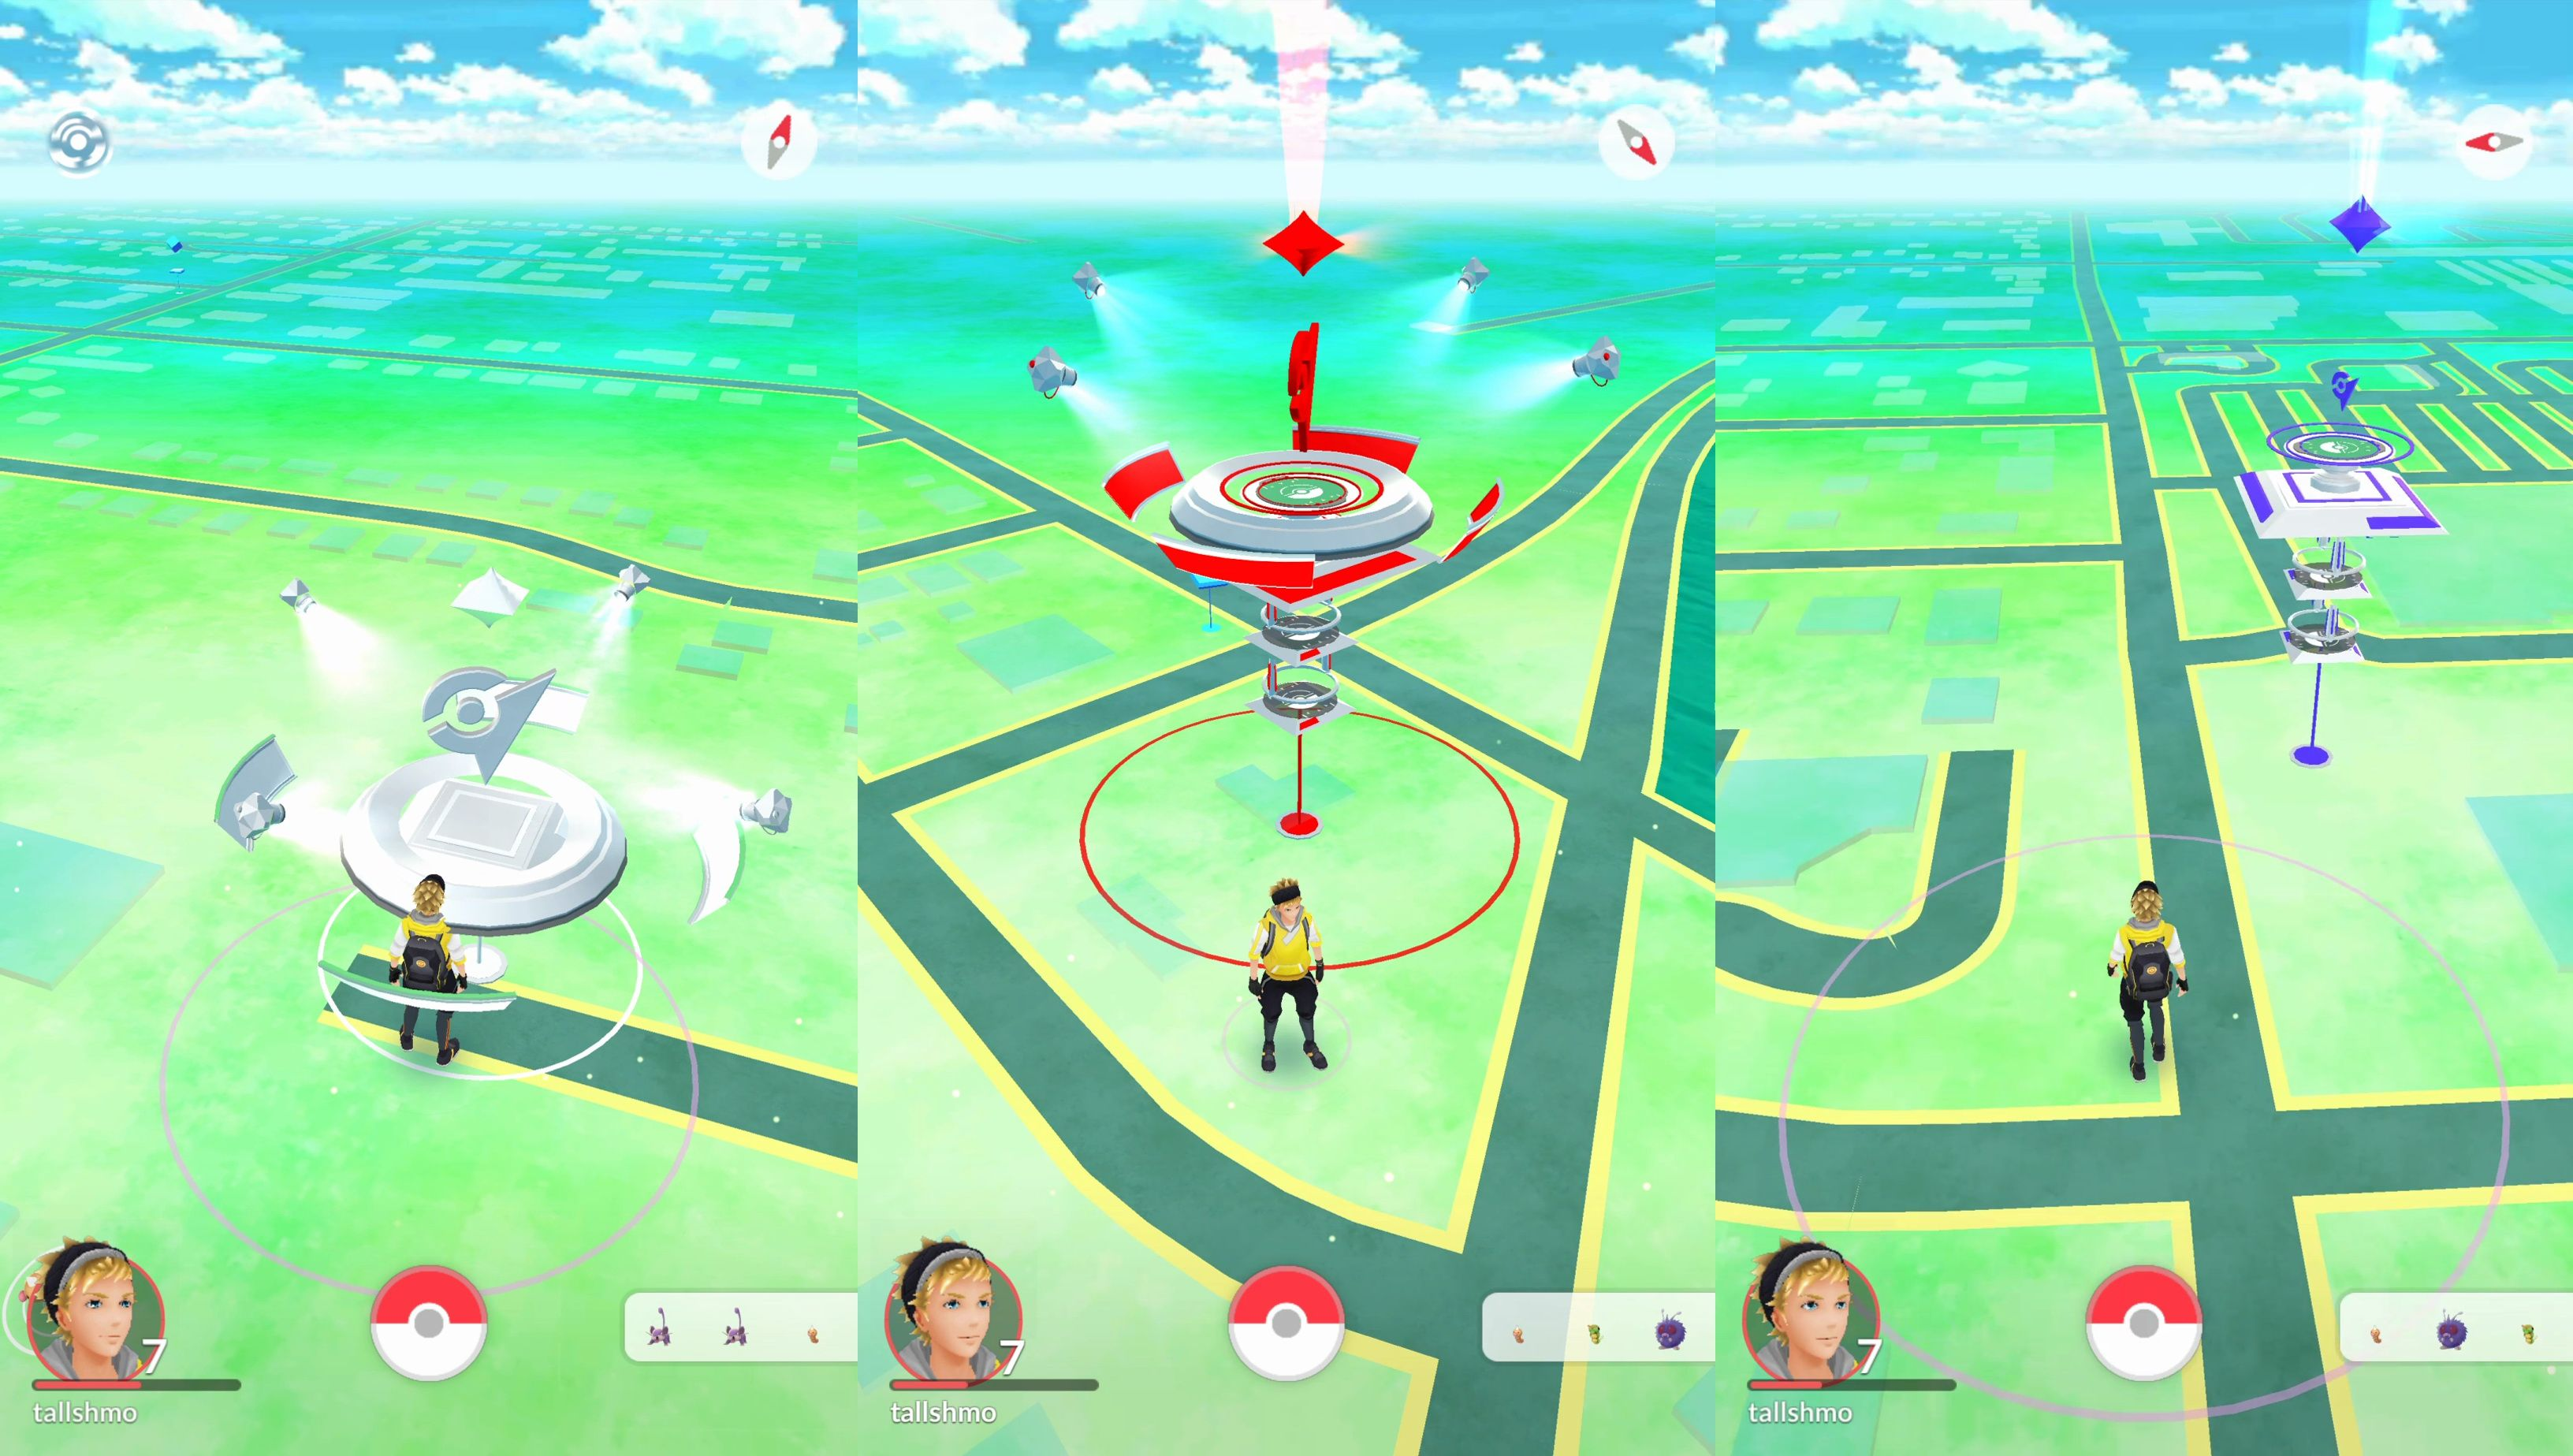
\includegraphics[width=\textwidth]{slike/Slika2.1.JPG} %veličina u odnosu na širinu linije
			\caption{Primjer karte u Pokemon GO}
			\label{fig:promjene1} %label mora biti drugaciji za svaku sliku
		\end{figure}
		
		\begin{figure}[H]
			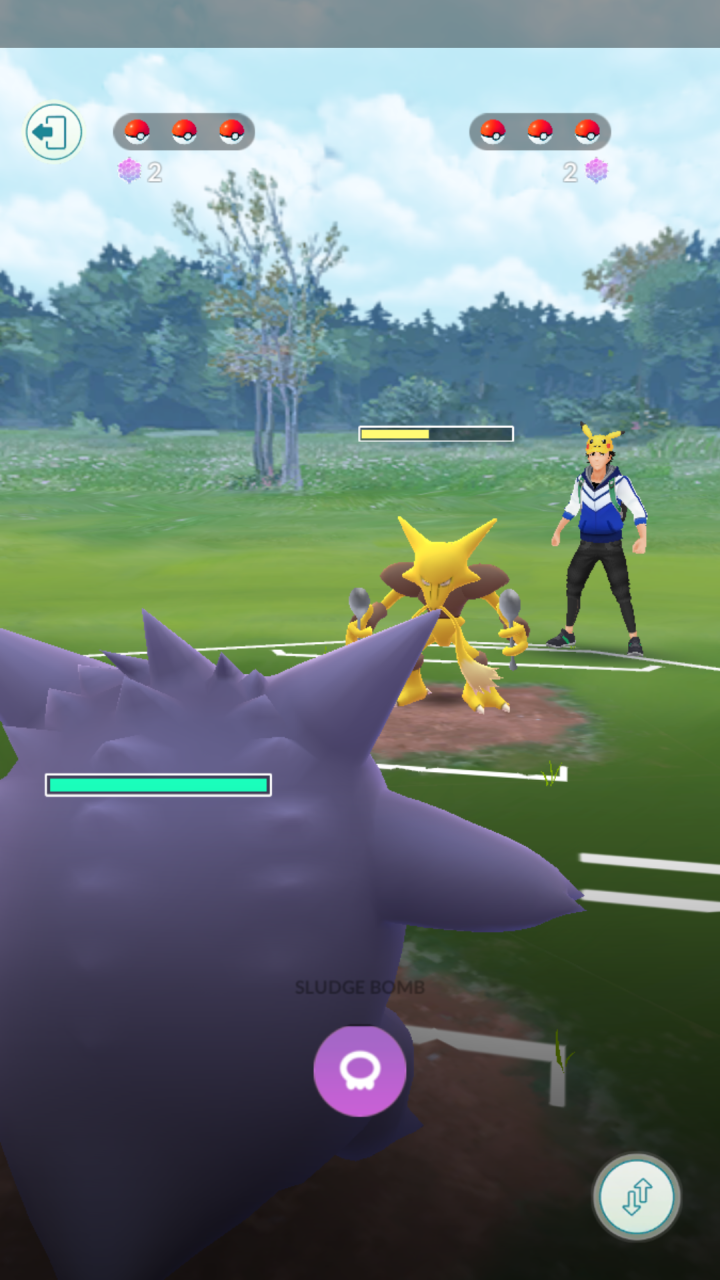
\includegraphics[scale=0.5]{slike/Slika2.2.PNG} %veličina u odnosu na širinu linije
			\centering
			\caption{Primjer borbe u Pokemon GO}
			\label{fig:promjene2} %label mora biti drugaciji za svaku sliku
		\end{figure}
		
		
		\eject
		
	